\documentclass[10pt]{beamer}

\usepackage[utf8]{inputenc}
\usepackage{float}
\usepackage[british]{babel}
\usepackage{amsmath, amsfonts, amssymb}
\usepackage{graphicx}
\usepackage{booktabs} 
\usepackage{tikz}
\usepackage{xcolor}

\usetheme{Madrid}
\usecolortheme{whale}
\setbeamertemplate{navigation symbols}{} 
\setbeamertemplate{headline}{}

\title[Processos Estocásticos II]{Trabalho Clusterização \\ Análise de Churn com K-Means e Hierárquico}
\author{Mateus Ribeiro Gomes}
\date{\today}

\begin{document}

\begin{frame}
    \titlepage
\end{frame}

% --- SEÇÃO 1: INTRODUÇÃO ---
\section{Introdução}

\begin{frame}{Contexto do Problema}
    \begin{itemize}
        \item \textbf{Objetivo:} Agrupar clientes com base em seu perfil de uso para identificar padrões de \textit{churn} (evasão).
        \item \textbf{Dataset:} 3150 amostras, 13 atributos e 1 de label (Churn).
        \item Todos os atributos, exceto o atributo de churn, representam
            dados agregados dos primeiros 9 meses. Os rótulos de churn
            refletem a situação dos clientes ao final de 12 meses.    
    \end{itemize}
    \vfill
    \begin{columns}
        \begin{column}{0.5\textwidth}
            \textbf{Atributos:}
            \begin{itemize}
                \item {Call Failure (número de falhas)}
                \item {Complains (binário)}
                \item {Subscription Lenght (meses)}
                \item {Seconds of Use}
                \item {Frequency of Use (número de calls)}
                \item {Frequency of SMS (número de sms's)}
                \item {Distinct Called Numbers}
            \end{itemize}
        \end{column}
        \begin{column}{0.5\textwidth}
            \begin{itemize}
                \item {Age Group(ordinal [1, 5])}
                \item {Charge Amount (ordinal [0, 9])}
                \item {Tariff Plan (binario: pré ou pós pago)}
                \item {Status (binário: ativo ou não)}
                \item {Customer Value}
                \item {Churn (binário)}
            \end{itemize}
        \end{column}
    \end{columns}
\end{frame}

\begin{frame}{Pairplot dos Dados}
    \begin{figure}
        \centering
        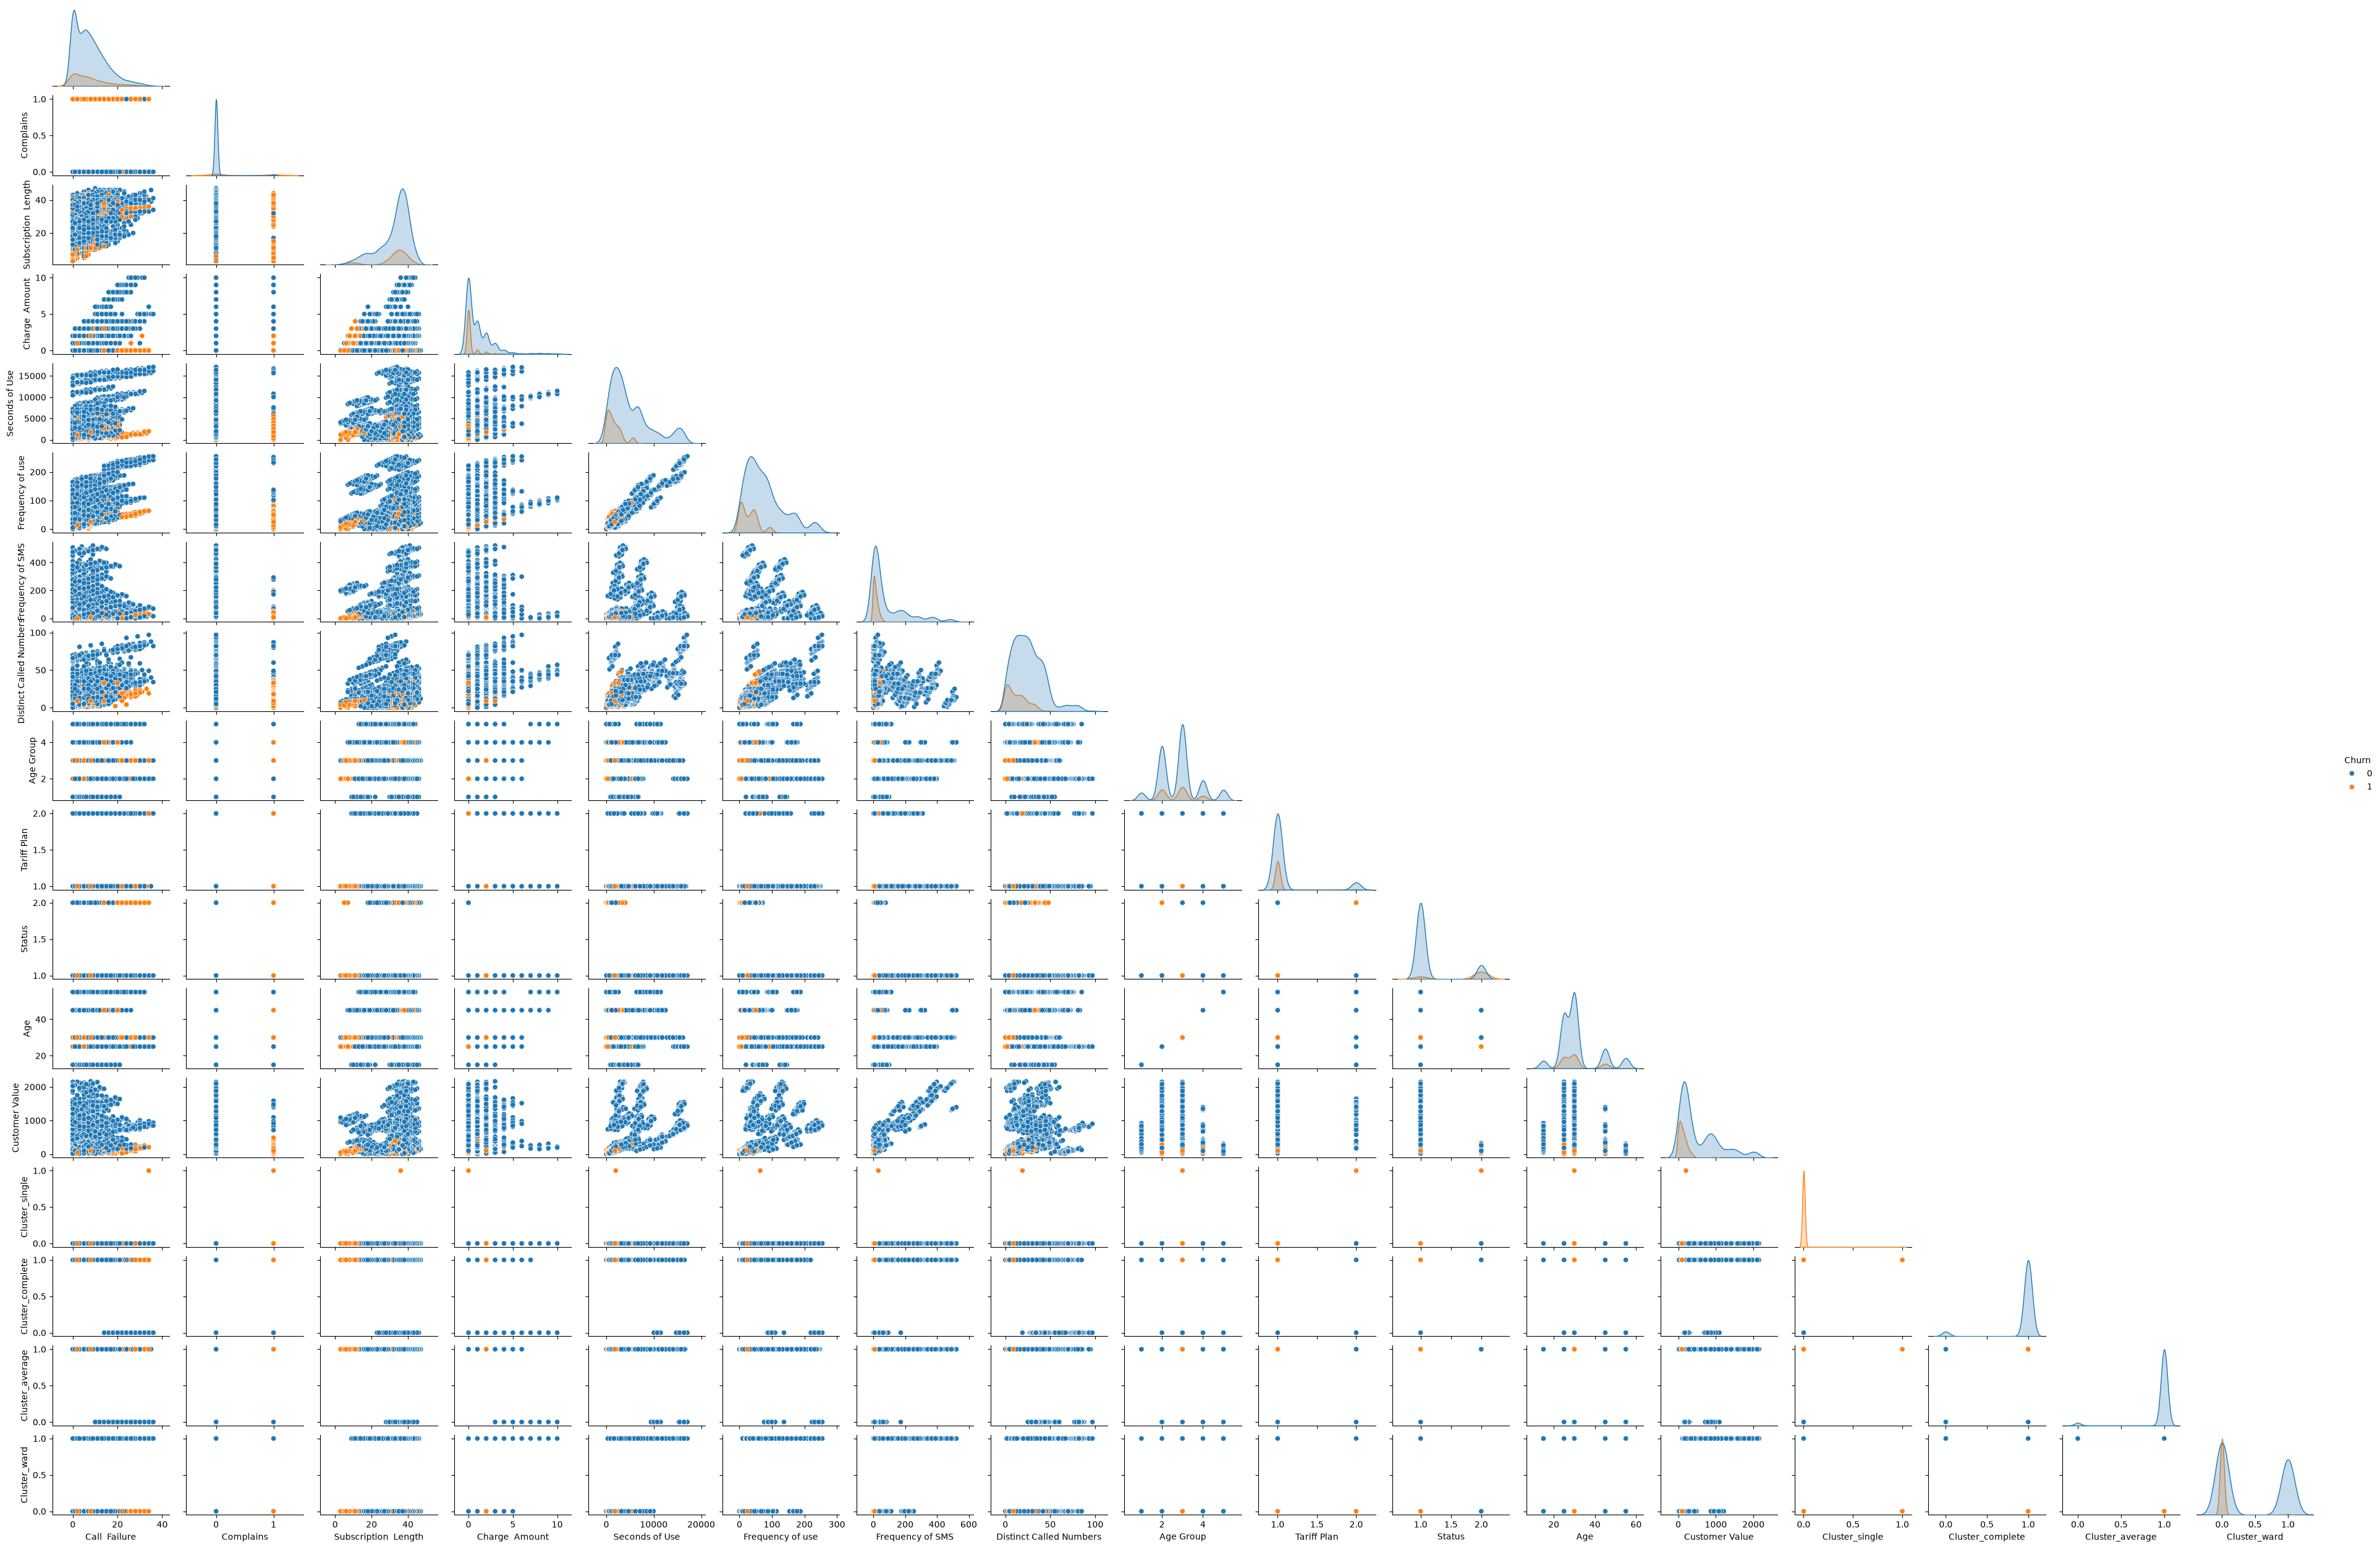
\includegraphics[width=1.0\textwidth]{images/pairplot.png}
        \caption{Pairplot dos dados colorido por Churn.}
    \end{figure}
\end{frame}

% --- SEÇÃO 2: PRÉ-PROCESSAMENTO ---
\section{Pré-processamento}

\begin{frame}{Padronização das Features}
    \begin{itemize}
        \item É necessário padronizar as features pois há atributos que possuem grande diferença na ordem de grandeza.
        \item Exemplo: \texttt{Seconds of Use} está na casa dos milhares, enquanto \texttt{Call Failure} está na casa das dezenas.
    \end{itemize}
    \vfill
    \begin{equation*}
        X_{\text{scaled}} = \frac{X - \mu}{\sigma}
    \end{equation*}
    \begin{block}{Explicação}
        Sem essa padronização, os algoritmos seriam "ingênuos", ou seja,  eles
        tratariam uma diferença de 1000 segundos de uso como 1000 vezes mais
        importante do que uma diferença de 1 falha de chamada, simplesmente por
        causa do valor numérico, e não da relevância estatística.
    \end{block}
\end{frame}

% --- SEÇÃO 3: K-MEANS ---
\section{K-Means}

\begin{frame}{Algoritmo K-Means}
    O algoritmo segue o seguinte fluxo:
    \begin{enumerate}
        \item Os centroides são inicializados de maneira aleatória.
        \item Calcula-se a distância de cada ponto para todos os centroides; cada ponto é atribuído ao que apresentar a menor distância.
        \item Calcula-se a média espacial dos pontos atribuídos a cada centroide.
        \item O novo centroide passa a ser esse valor da média calculada.
        \item Repete-se o processo até convergência (centroides param apresentar mudança considerável) ou até o limite máximo de iterações.
    \end{enumerate}
\end{frame}

\begin{frame}{Métricas de Distância}
    Três métricas de distância foram testadas:
    \vfill
    \begin{block}{Distância Euclidiana}
        \begin{equation*}
            d(x, y) = \sqrt{\sum_{i} (x_i - y_i)^2}
        \end{equation*}
    \end{block}
    \begin{block}{Distância de Mahalanobis}
        \begin{equation*}
            d(x, y) = \sqrt{(x - y)^T \Sigma^{-1} (x - y)}
        \end{equation*}
    \end{block}
    \begin{block}{Distância de Manhattan}
        \begin{equation*}
            d(x, y) = \sum_{i} |x_i - y_i|
        \end{equation*}
    \end{block}
\end{frame}

\begin{frame}{PCA para Visualização 2D}
    \begin{itemize}
        \item Para visualizar os clusters em 2 dimensões, utilizou-se Análise de Componentes Principais (PCA).
        \item O PCA foi aplicado apenas para visualização, os modelos foram treinados com a dimensão original (13 atributos).
        \item A PC1 e a PC2 apresentaram $\approx 50\%$ da variância dos dados.
    \end{itemize}
\end{frame}

% --- SEÇÃO 4: MÉTODO DO COTOVELO ---
\section{Método do Cotovelo}

\begin{frame}{Cotovelo - Distância Euclidiana}
    \begin{itemize}
        \item A curva de inércia apresenta uma inflexão clara em $k=2$.
        \item A redução da inércia após $k=2$ torna-se gradual.
    \end{itemize}
    \vfill
    \begin{figure}
        \centering
        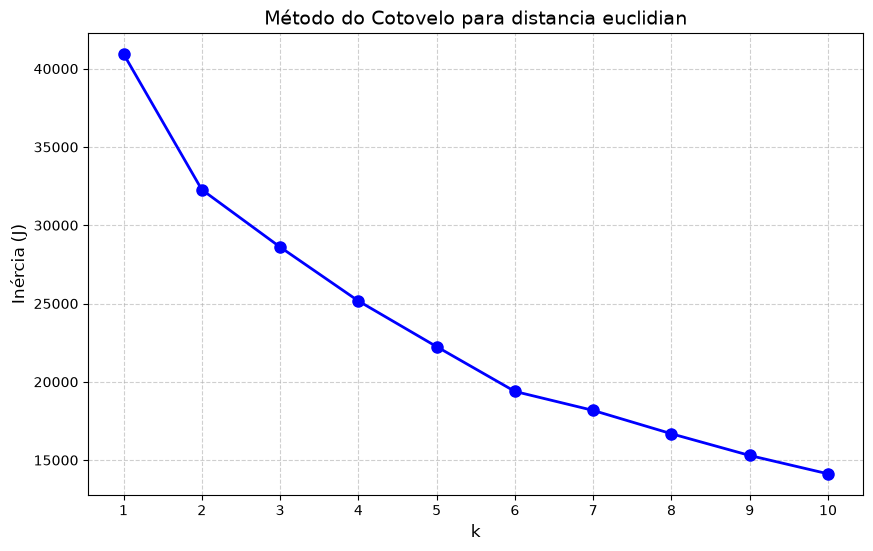
\includegraphics[width=0.7\textwidth]{images/cotovelo_euclid.png}
    \end{figure}
\end{frame}

\begin{frame}{Cotovelo - Distância de Mahalanobis}
    \begin{itemize}
        \item Comportamento linear, sem pontos de inflexão acentuados.
        \item Ausência de um ``cotovelo'' definido indica que o modelo não encontra uma estrutura de separação otimizada.
        \item A métrica se apresenta como ineficaz para esta base de dados.
    \end{itemize}
    \vfill
    \begin{figure}
        \centering
        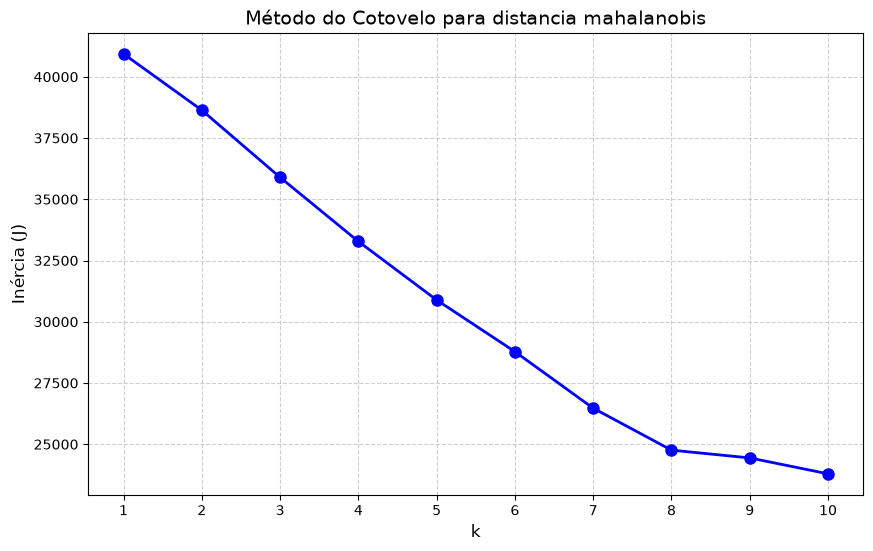
\includegraphics[width=0.7\textwidth]{images/cotovelo_mahala.png}
    \end{figure}
\end{frame}

\begin{frame}{Cotovelo - Distância de Manhattan}
    \begin{itemize}
        \item Comportamento semelhante ao Euclidiano, com inflexão marcante em $k=2$.
        \item A partir de $k=2$, a inclinação diminui significativamente.
    \end{itemize}
    \vfill
    \begin{figure}
        \centering
        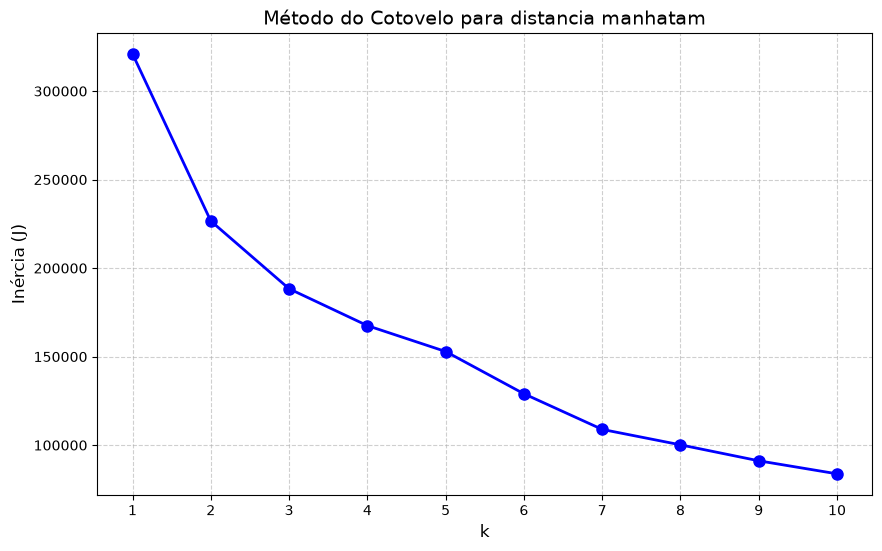
\includegraphics[width=0.7\textwidth]{images/cotovelo_manh.png}
    \end{figure}
\end{frame}

% --- SEÇÃO 5: VISUALIZAÇÃO DOS CLUSTERS ---
\section{Visualização dos Clusters}

\begin{frame}{K-Means - Euclidiana $k=2$}
    \begin{itemize}
        \item A distância Euclidiana apresentou bom desempenho na separação dos clusters.
    \end{itemize}
    \vfill
    \begin{figure}
        \centering
        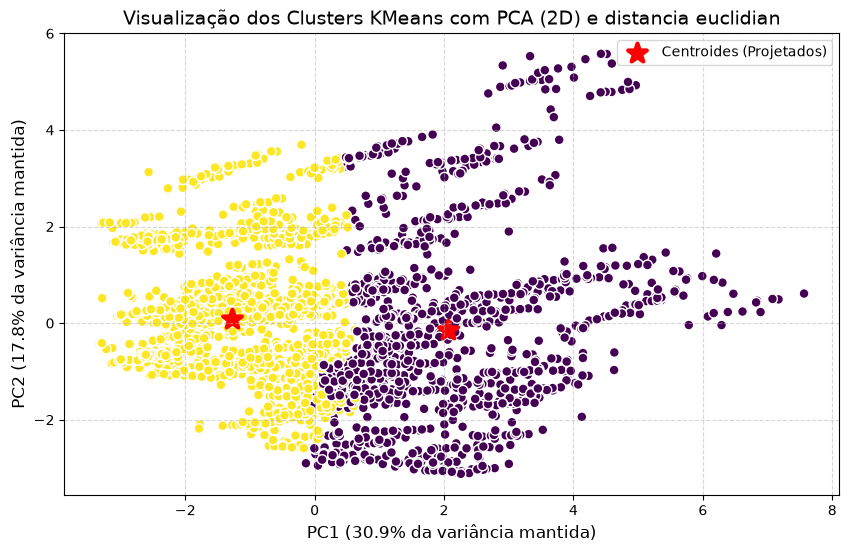
\includegraphics[width=0.7\textwidth]{images/kmeans_euclidian_k2.png}
    \end{figure}
\end{frame}

\begin{frame}{K-Means - Euclidiana $k=3$}
    \begin{figure}
        \centering
        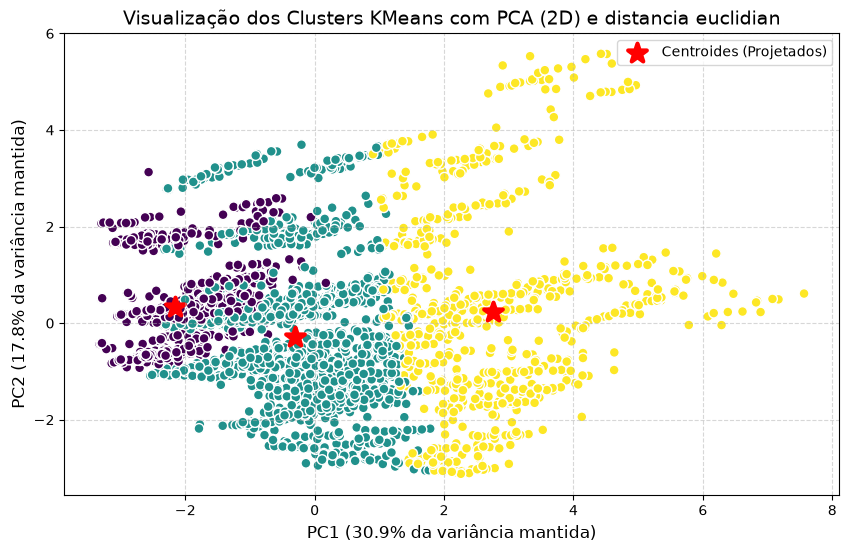
\includegraphics[width=0.7\textwidth]{images/kmeans_euclidian_k3.png}
    \end{figure}
\end{frame}

\begin{frame}{K-Means - Mahalanobis $k=2$}
    \begin{itemize}
        \item Separação fraca entre os clusters.
    \end{itemize}
    \vfill
    \begin{figure}
        \centering
        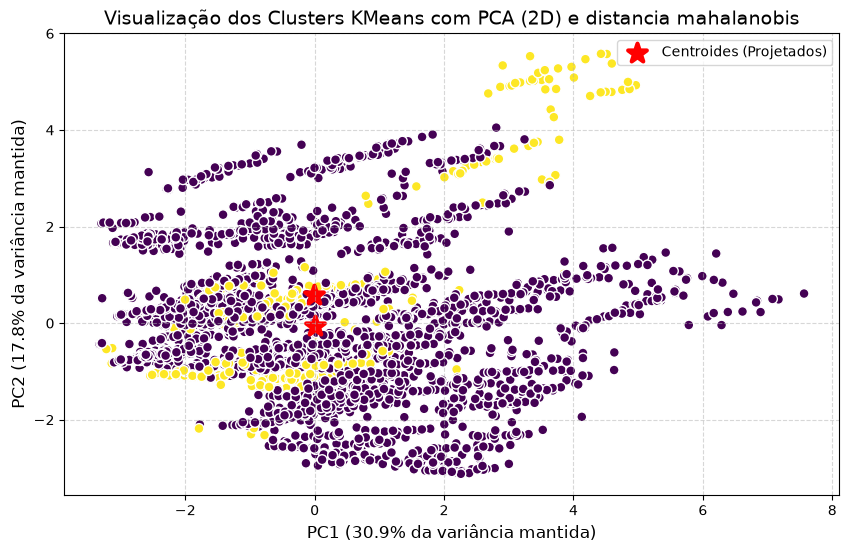
\includegraphics[width=0.7\textwidth]{images/kmeans_mahala_k2.png}
    \end{figure}
\end{frame}

\begin{frame}{K-Means - Manhattan $k=2$}
    \begin{itemize}
        \item A distância de Manhattan também apresentou boa separação.
    \end{itemize}
    \vfill
    \begin{figure}
        \centering
        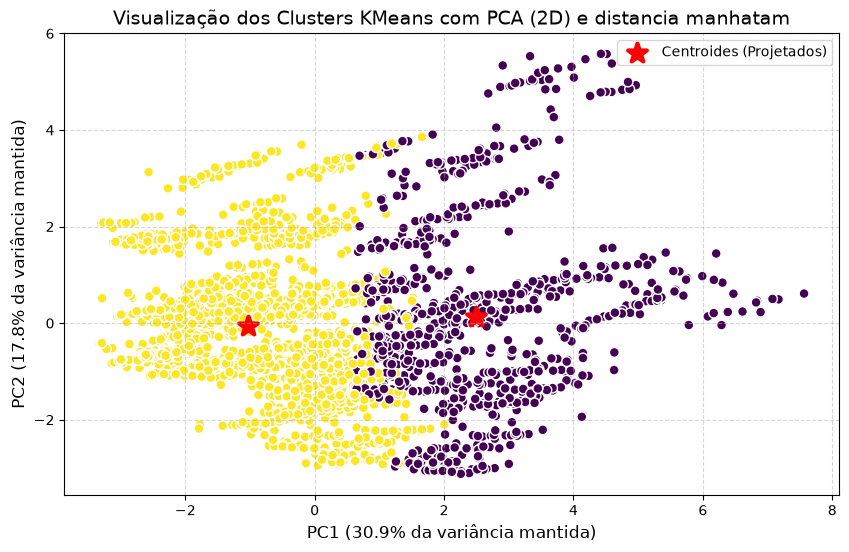
\includegraphics[width=0.7\textwidth]{images/kmeans_manh_k2.png}
    \end{figure}
\end{frame}

\begin{frame}{K-Means - Manhattan $k=3$}
    \begin{itemize}
        \item Curiosamente, quando utilizada com K = 3, a métrica de manhatam demonstrou uma capacidade
            razoável de clustrização do espaço.
    \end{itemize}
    \vfill
    \begin{figure}
        \centering
        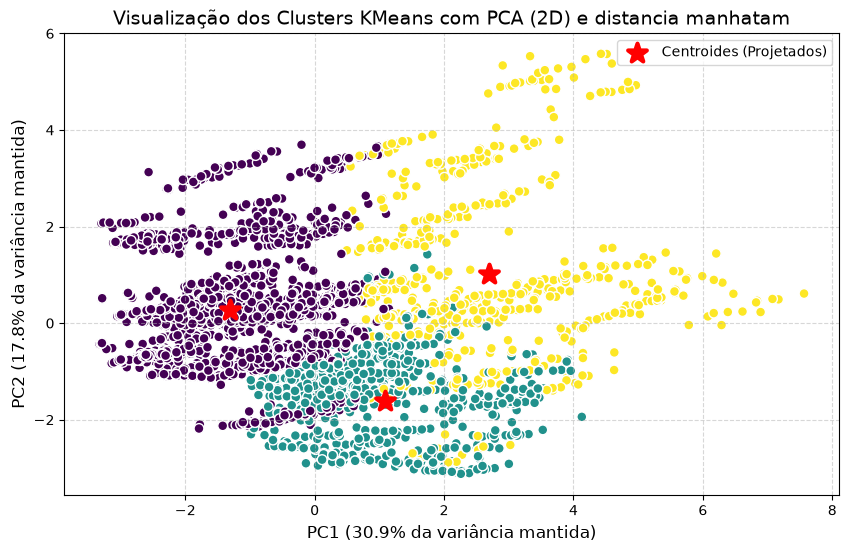
\includegraphics[width=0.7\textwidth]{images/kmeans_manh_k3.png}
    \end{figure}
\end{frame}

% --- SEÇÃO 6: DIFERENTES INICIALIZAÇÕES ---
\section{Diferentes Inicializações}

\begin{frame}{Impacto de Diferentes Inicializações}
    \begin{itemize}
        \item O K-Means é sensível à inicialização dos centroides, podendo convergir para mínimos locais.
        \item Testamos múltiplas inicializações (sem seed) para 2 cenários gerados:
        \begin{itemize}
            \item Euclidiana $k=2$ (melhor desempenho visual)
            \item Manhattan $k=3$ (comportamento curioso)
        \end{itemize}
    \end{itemize}
\end{frame}

\begin{frame}{Euclidiana $k=2$ - Diferentes Inicializações dos Centroides}
    \begin{figure}
        \centering
        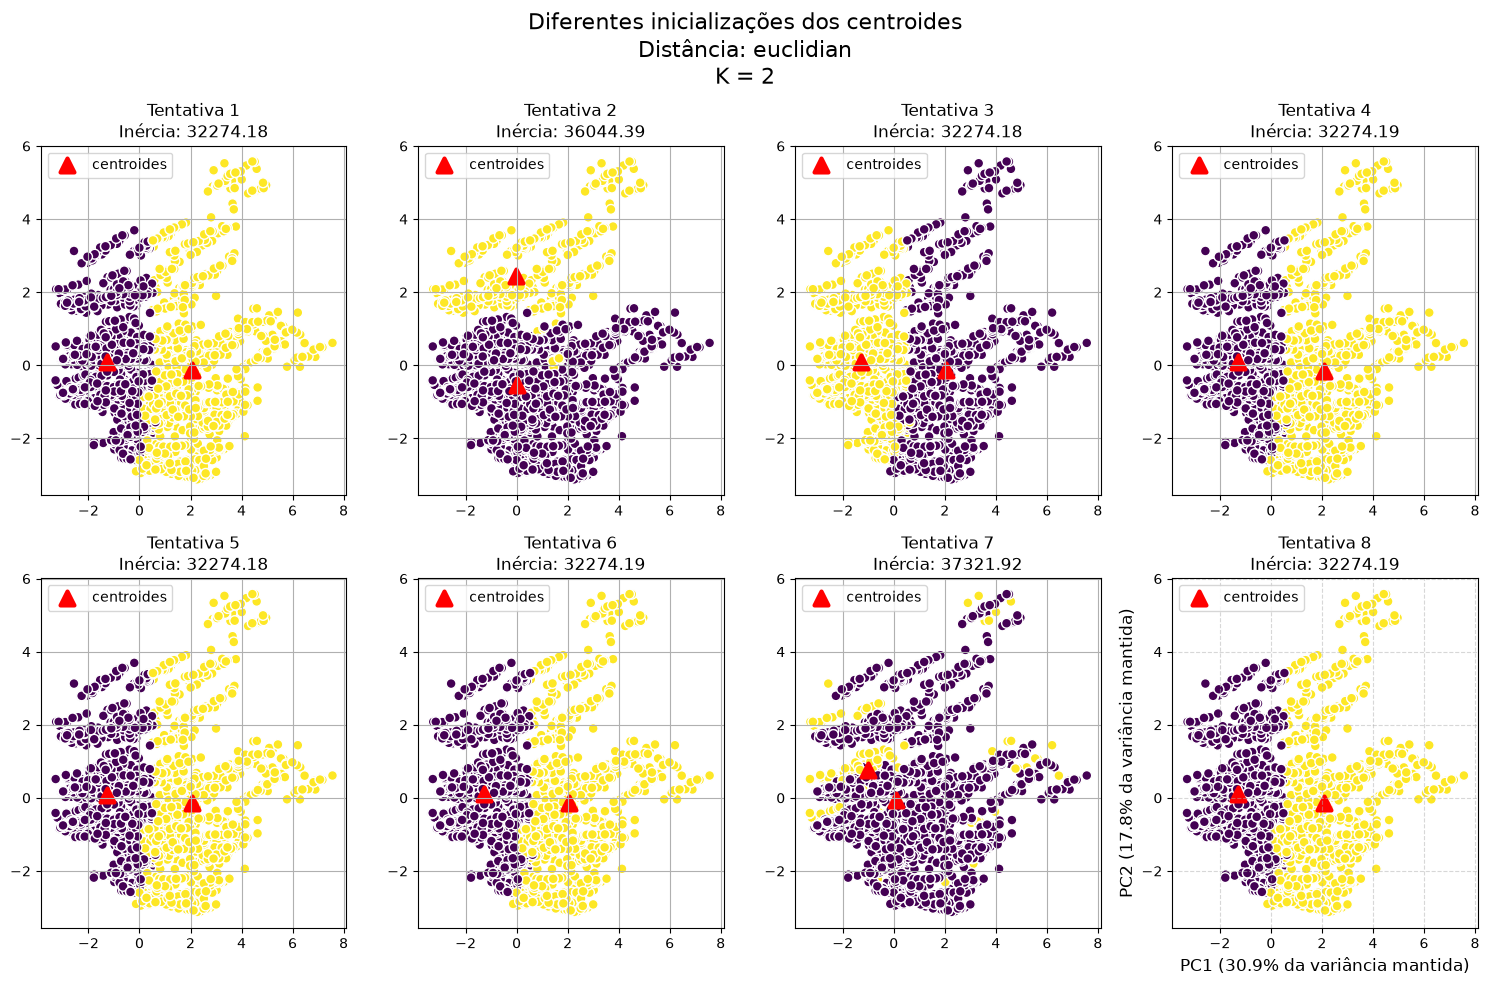
\includegraphics[width=0.85\textwidth]{images/diferentes_centroides_euclid.png}
    \end{figure}
\end{frame}

\begin{frame}{Manhattan $k=3$ - Diferentes Inicializações dos Centroides}
    \begin{figure}
        \centering
        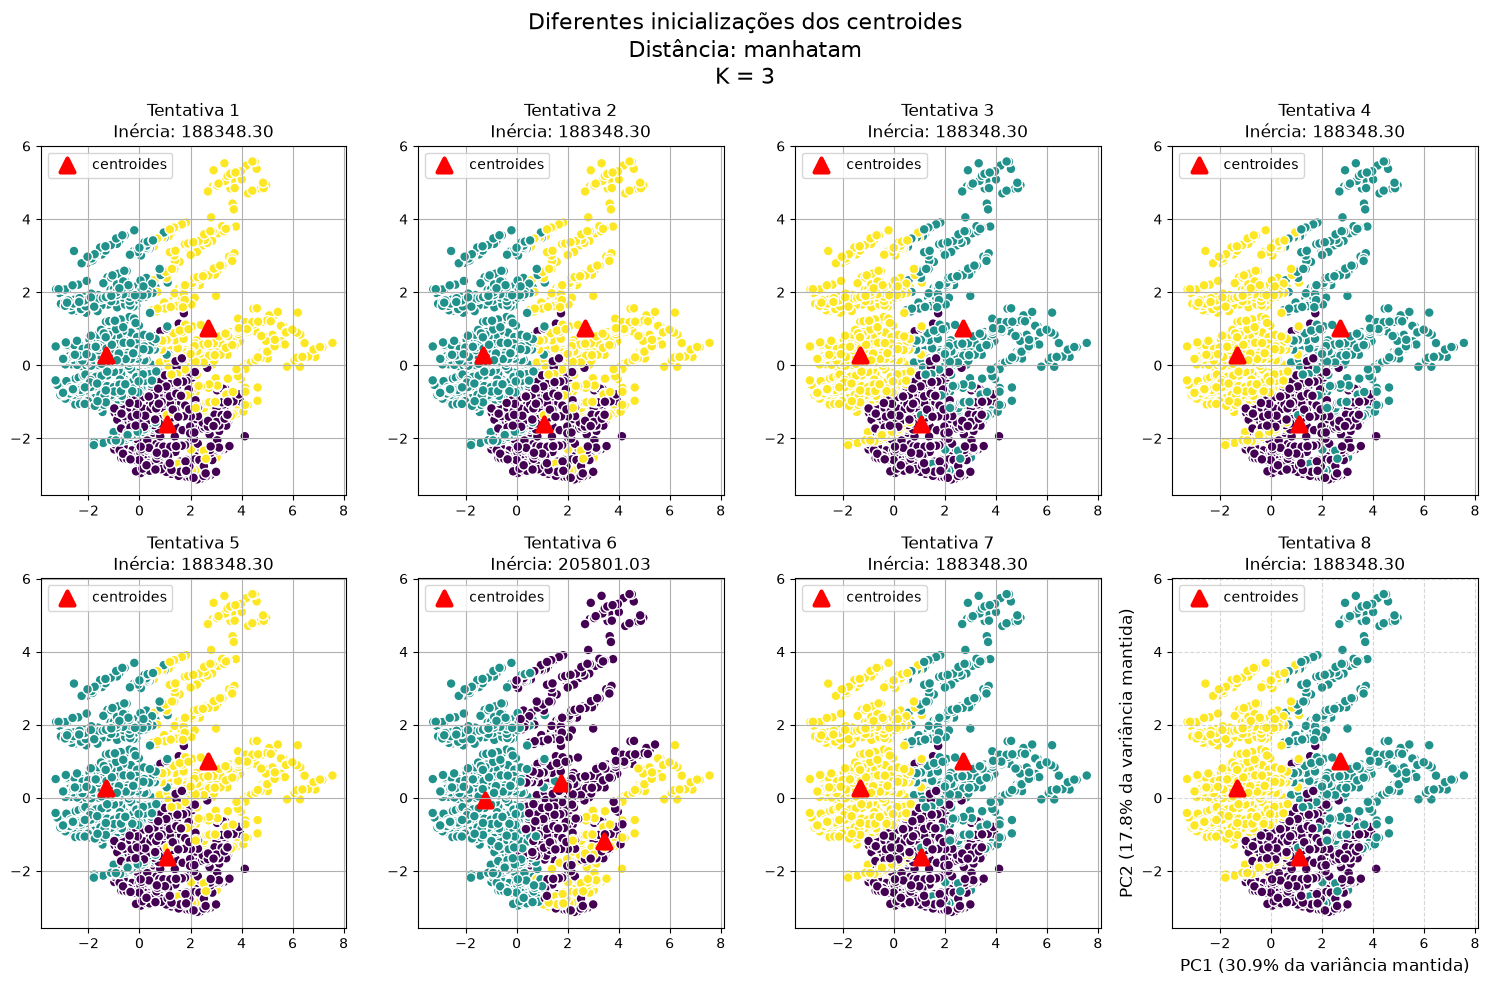
\includegraphics[width=0.85\textwidth]{images/diferentes_centroides_manh.png}
    \end{figure}
\end{frame}

% --- SEÇÃO 7: ANÁLISE DE CHURN (K-MEANS) ---
\section{Análise de Churn - K-Means}

\begin{frame}{Probabilidade de Churn por Cluster}
    \centering
    \footnotesize
    \begin{tabular}{lcc}
        \toprule
        \textbf{Métrica} & \textbf{Cluster} & \textbf{Prob. Churn} \\
        \midrule
        Euclidiana $k=2$ & 0 & 0.75\% \\
        & 1 & 25.03\% \\
        \midrule
        Mahalanobis $k=2$ & 0 & 15.30\% \\
        & 1 & 19.27\% \\
        \midrule
        Manhattan $k=2$ & 0 & 0.33\% \\
        & 1 & 22.09\% \\
        \midrule
        Manhattan $k=3$ & 0 & 26.18\% \\
        & 1 & 1.58\% \\
        & 2 & 0.49\% \\
        \bottomrule
    \end{tabular}
\end{frame}

\begin{frame}{Conclusões - KMeans}
    \begin{block}{Euclidiana}
        Bom desempenho: Cluster 0 com 0.75\% e Cluster 1 com 25.03\% de Churn. Adequação da métrica à geometria dos dados.
    \end{block}
    \begin{block}{Mahalanobis}
        Desempenho limitado (15.30\% vs 19.27\%). 

        A premissa de normalidade multivariada não é atendida pelos dados (distribuições não normais e assimétricas).
    \end{block}
    \begin{block}{Manhattan}
        Boa abordagem: com $k=2$ (0.33\% vs 22.09\%). 

        Com $k=3$, revela uma possível terceira categoria de risco moderado, isolando melhor o segmento de alta evasão.
    \end{block}
\end{frame}

% --- SEÇÃO 8: HIERÁRQUICO AGLOMERATIVO ---
\section{Hierárquico Aglomerativo}

\begin{frame}{Algoritmo Hierárquico Aglomerativo (Bottom-Up)}
    \begin{enumerate}
        \item Inicia-se com pontos individuais (cada ponto é seu próprio cluster).
        \item Calcula-se a distância entre todos os pares de clusters.
        \item Identificam-se os dois clusters mais próximos e unem-os.
        \item Recalculam-se as distâncias entre o novo cluster e os demais.
        \item Repete-se até que todos os pontos estejam em um único cluster.
    \end{enumerate}
\end{frame}

\begin{frame}{Métodos de Linkage}
    Assuma um cluster $u$ resultante da junção de dois outros clusters $s$ e $t$, 
    e $v$ qualquer outro cluster diferente:
    \vfill
    \begin{itemize}
        \item \textbf{Single:}
        \begin{equation*}
            d(u,v) = \min(\operatorname{dist}(u[i], v[j]))
        \end{equation*}
        \item \textbf{Complete:}
        \begin{equation*}
            d(u,v) = \max(\operatorname{dist}(u[i], v[j]))
        \end{equation*}
        \item \textbf{Average:}
        \begin{equation*}
            d(u,v) = \sum_{ij} \frac{\operatorname{dist}(u[i], v[j])}{|u| \cdot |v|}
        \end{equation*}
        \item \textbf{Ward:}
        \begin{equation*}
            d(u,v) = \sqrt{\frac{|v| + |s|}{T} d(v,s)^2 + \frac{|v| + |t|}{T} d(v,t)^2 - \frac{|v|}{T} d(s,t)^2}
        \end{equation*}
            onde $T = |v| + |s| + |t|$ e $|*|$ é o operador de cardinalidade.
    \end{itemize}
\end{frame}

\begin{frame}{Dendrogramas - 4 Métodos de Linkage}
    \begin{figure}
        \centering
        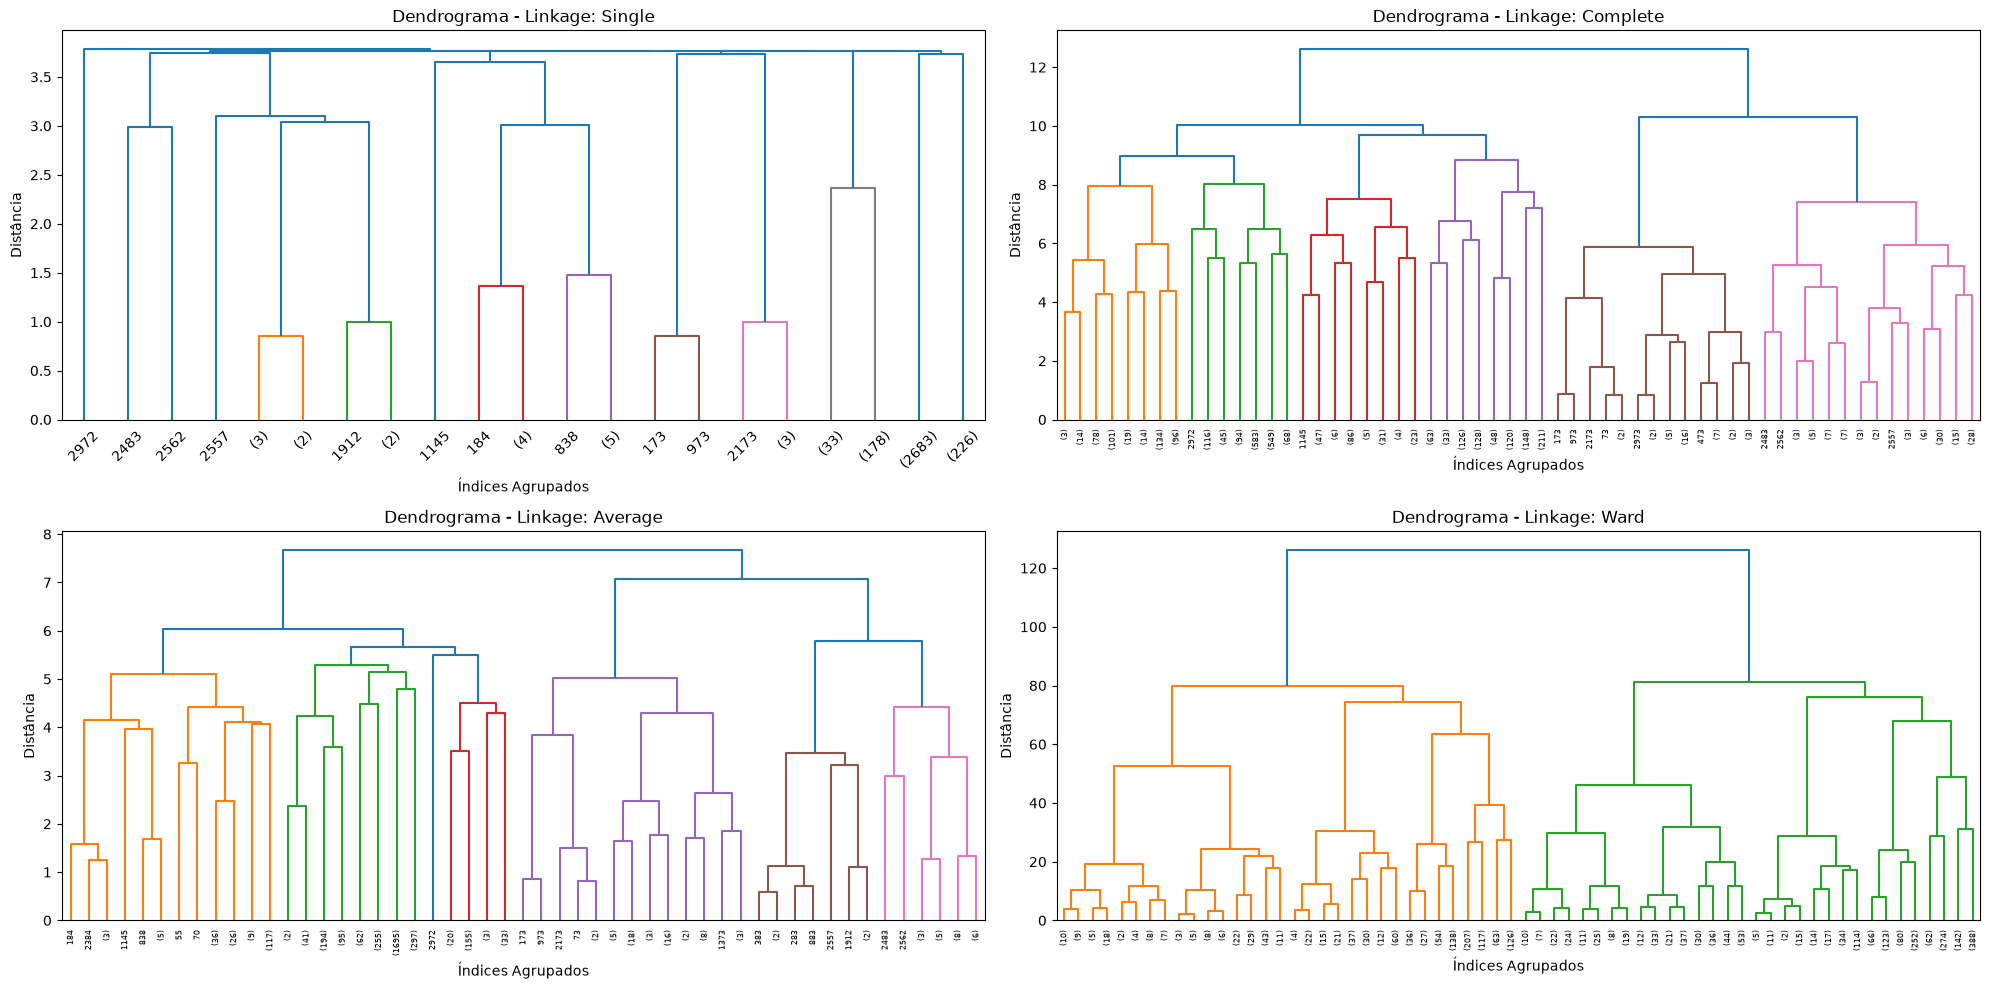
\includegraphics[width=0.9\textwidth]{images/dendogramas.png}
        \caption{Dendrogramas para os métodos Single, Complete, Average e Ward.}
    \end{figure}
\end{frame}

\begin{frame}[shrink=10]{Análise dos métodos}
    \begin{block}{Single}
        \begin{itemize}
            \item Apresenta um forte efeito de "escada", unindo os dados de forma sequencial.
            \item É a topologia que se demonstrou menos adequada para a clusterização de perfis nesta base de dados.
        \end{itemize}
    \end{block}

    \begin{block}{Complete}
        \begin{itemize}
            \item Gera uma árvore com muitas sub-ramificações que demoram mais para se juntarem.
            \item Pode dividir grupos que naturalmente pertenceriam juntos devido à sensibilidade às extremidades dos clusters.
        \end{itemize}
    \end{block}

    \begin{block}{Average}
        \begin{itemize}
            \item Atua como um meio-termo matemático entre os extremos dos métodos Single e Complete.
            \item Agrupa os clientes calculando a distância média entre todos os pares.
            \item Constrói uma topologia útil, mas ainda preserva galhos irregulares na base da árvore.
        \end{itemize}
    \end{block}

    \begin{block}{Ward}
        \begin{itemize}
            \item Agrupa os clientes minimizando a variância interna, gerando os clusters mais homogêneos possíveis.
            \item Produz ramificações espessas e simétricas, facilitando a identificação visual do ponto de corte ideal ($k$).
            \item É o método que se demonsrou mais adequado ao conjunto para isolar as fronteiras do risco de churn.
        \end{itemize}
    \end{block}

\end{frame}
   

\begin{frame}{Clusters Hierárquicos com PCA}
    \begin{figure}
        \centering
        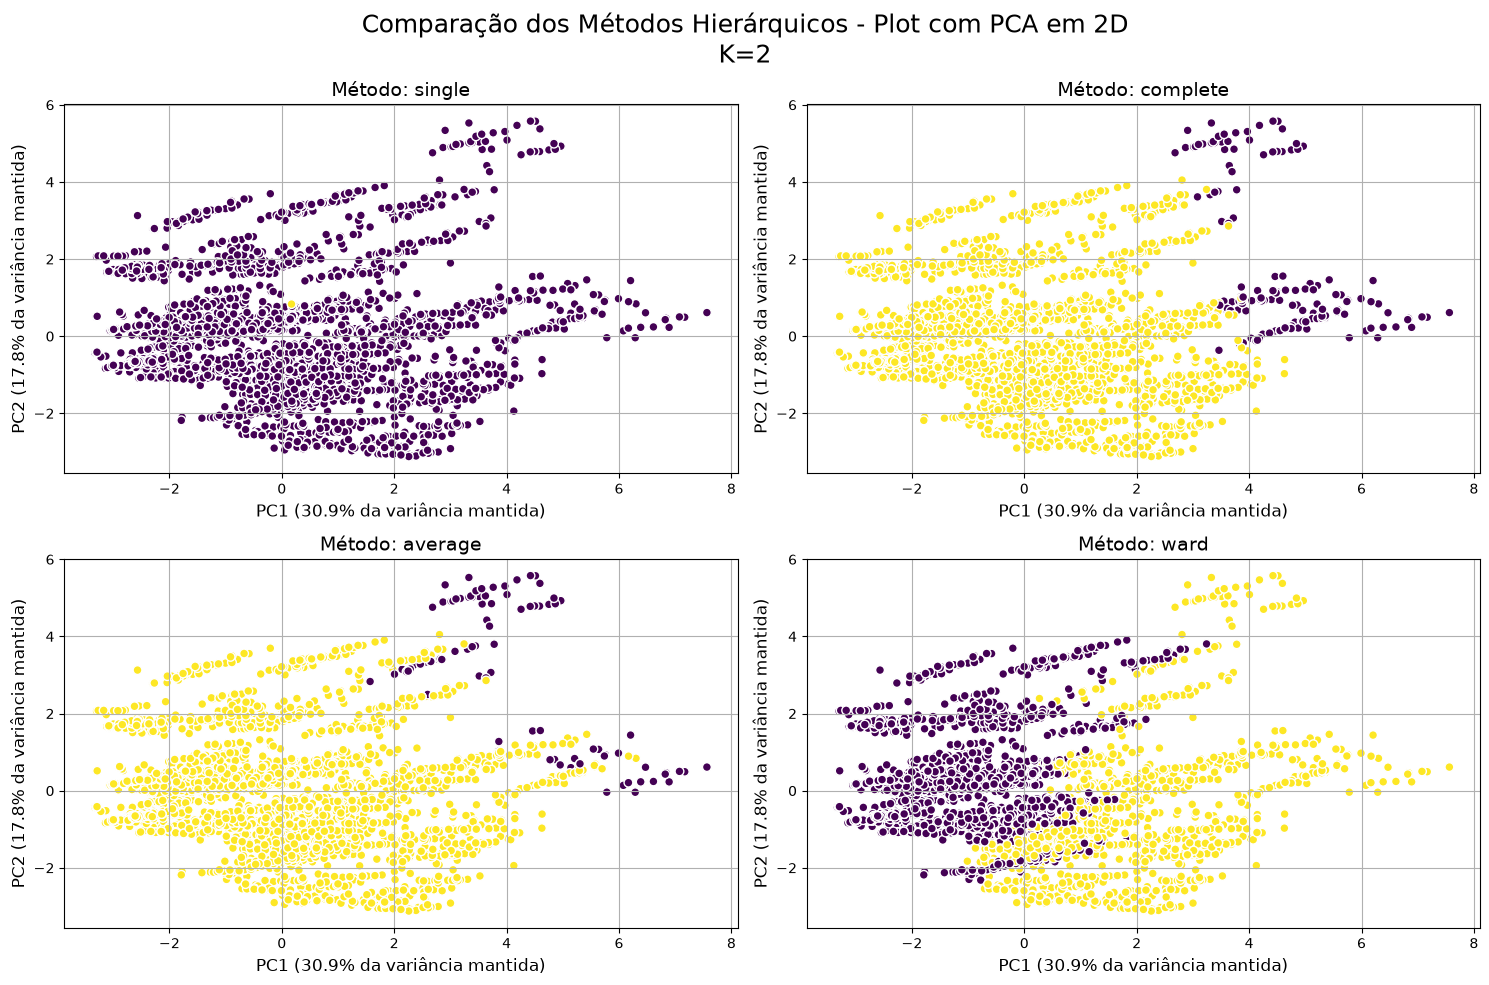
\includegraphics[width=0.85\textwidth]{images/hierarquico_clusters.png}
        \caption{Visualização dos clusters hierárquicos projetados em 2D com PCA.}
    \end{figure}
\end{frame}

% --- SEÇÃO 9: ANÁLISE DE CHURN (HIERÁRQUICO) ---
\section{Análise de Churn --- Hierárquico}

\begin{frame}{Probabilidade de Churn por Método de Linkage}
    \centering
    \footnotesize
    \begin{tabular}{lcc}
        \toprule
        \textbf{Método} & \textbf{Cluster} & \textbf{Prob. Churn} \\
        \midrule
        Single & 0 & 15.69\% \\
        & 1 & 100.00\% \\
        \midrule
        Complete & 0 & 0.00\% \\
        & 1 & 16.53\% \\
        \midrule
        Average & 0 & 0.00\% \\
        & 1 & 16.20\% \\
        \midrule
        Ward & 0 & 24.56\% \\
        & 1 & 0.52\% \\
        \bottomrule
    \end{tabular}
\end{frame}

\begin{frame}{Conclusões - Hierárquico}
    \begin{itemize}
        \item \textbf{Single:} Cluster 1 com 100\% de Churn, mas apenas 1 cliente, efeito de \textit{chaining}.
        \item \textbf{Complete:} Cluster 0 com 0\% de Churn e Cluster 1 com 16.53\%, boa separação.
        \item \textbf{Average:} Resultado similar ao Complete (0\% e 16.20\%).
        \item \textbf{Ward:} Cluster 0 com 24.56\% e Cluster 1 com 0.52\%, boa separação também.
        \item Ward e Complete apresentam a melhor separação de risco de Churn.
    \end{itemize}
\end{frame}

% --- SEÇÃO 10: CONCLUSÃO FINAL ---
\section{Conclusão}

\begin{frame}{Conclusão Final Sobre os Métodos}
    \begin{itemize}
        \item \textbf{K-Means com distância Euclidiana ($k=2$) e Manhattan ($k=2$)} são as abordagens mais eficazes para segmentar clientes por risco de Churn.
        \item \textbf{Mahalanobis} mostrou-se inadequada para este conjunto de dados devido à não normalidade.
        \item \textbf{Hierárquico com Ward} também apresenta boa separação espacial.
    \end{itemize}
\end{frame}

\begin{frame}{Perfil de clientes}

    \begin{table}[htbp]
        \centering
        \caption{Perfil Médio de Consumo por Cluster (K-Médias Euclidiana, $k=2$)}
        \label{tab:perfil_consumo_k2}
        \begin{tabular}{lrr}
        \toprule
        \textbf{Variável} & \textbf{Cluster 0} & \textbf{Cluster 1} \\
        \midrule
        Call Failure            & 11.63   & 5.14    \\
        Complains               & 0.02    & 0.11    \\
        Subscription Length     & 33.96   & 31.66   \\
        Charge Amount           & 1.89    & 0.35    \\
        Seconds of Use          & 8167.33 & 2174.11 \\
        Frequency of use        & 119.25  & 38.49   \\
        Frequency of SMS        & 146.46  & 27.59   \\
        Distinct Called Numbers & 35.91   & 15.80   \\
        Age Group               & 2.89    & 2.79    \\
        Tariff Plan             & 1.18    & 1.02    \\
        Status                  & 1.00    & 1.40    \\
        Age                     & 31.59   & 30.63   \\
        Customer Value          & 908.68  & 198.70  \\
        Churn                   & 0.0075    & 0.25    \\
        \bottomrule
        \end{tabular}
    \end{table}
\end{frame}

\begin{frame}{Comportamento de usuários}
    \begin{itemize}
        \item Podemos ver que os clientes que possuem alto consumo estão classificados no
            cluster 0, o qual apresenta apenas 0.75\% de churn.

        \item O cluster 0 apresenta um perfil empresarial, dado a grande
            quantidade de números distintos apresentada, além de apresentar um
            valor baixo de churn mesmo com uma quantidade razoável de falhas,
            também mostra um grande valor agregado de cliente.


        \item O cluster 1 apresenta um perfil de usuários móvel, dado um menor
            valor agregado de cliente, uma taxa maior de reclamações, uma
            frequência de uso bem menor e um plano de tarifa mais próximo do
            pré pago.
    \end{itemize}

\end{frame}

\begin{frame}{Analisando com dados não padronizados}
    
    \begin{figure}
        \centering
        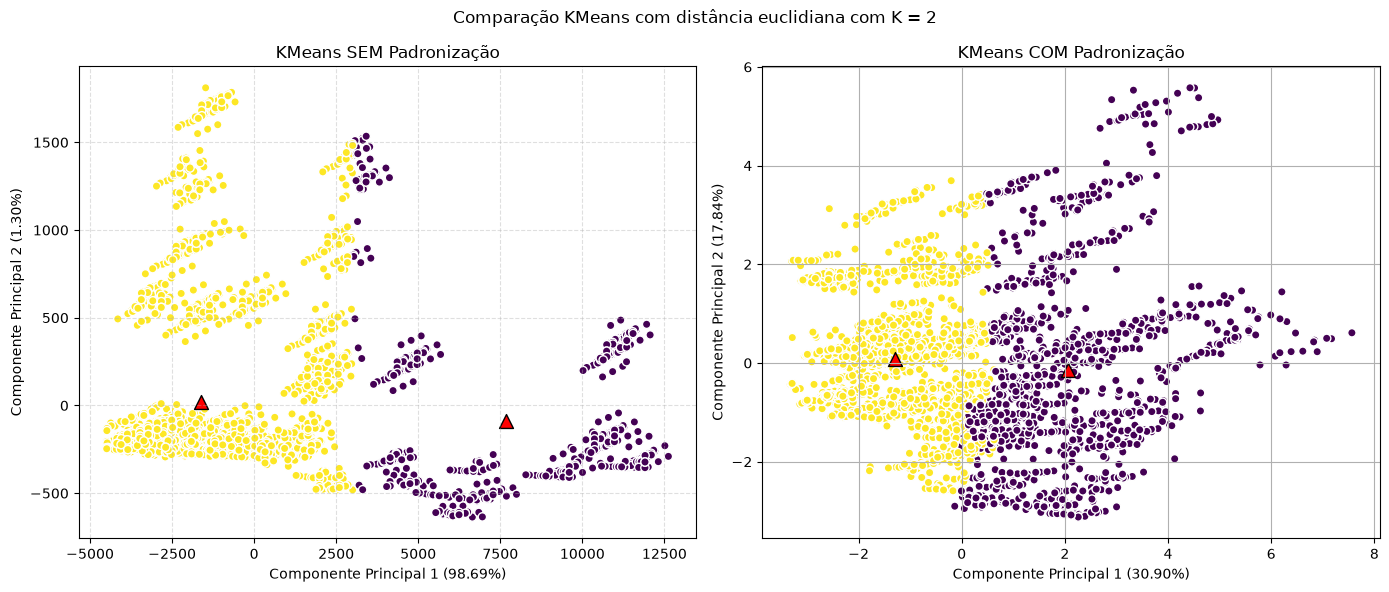
\includegraphics[width=0.85\textwidth]{images/comparacao_padronizacao.png}
    \end{figure}

    \begin{itemize}
        \item A variável \textit{Seconds of Use} (na casa dos milhares)
            passa a monopolizar o cálculo da distância, anulando o peso das
            demais métricas.
        \item Sem a padronização, o modelo ignora atributos de menor escala
            , porém essenciais para prever o risco (como
            \textit{Complains} e  \textit{Call Failure}).
        \item Ou seja, o algoritmo atuou mais como um "Separador de Tempo de Uso"
    \end{itemize}

\end{frame}

% --- Slide Final ---
\begin{frame}
    \centering
    \Huge Obrigado pela atenção! \\
    \vfill
    \Large Dúvidas?
\end{frame}

\end{document}
